% !Mode:: "TeX:UTF-8:Soft"
\ifx \allfiles \undefined
\documentclass[a4paper,12pt,twoside]{book}
%\usepackage{CJKutf8}
\usepackage[T1]{fontenc}
\usepackage{pifont}
\usepackage{graphicx}
\usepackage{capt-of}
\usepackage{color}
\usepackage{amsmath}
\newcommand{\linuxcommand}[1]{\texttt{\textcolor{blue}{\$ #1 \Pisymbol{psy}{191}}}}
\newcommand{\op}[1]{\textcolor{blue}{-#1}}
\newcommand{\hotkey}[1]{\framebox{#1}}
\newenvironment{screen}{\sffamily}{\rmfamily}
\newcommand{\tabincell}[2]{\begin{tabular}{@{}#1@{}}#2\end{tabular}}

\begin{document}
%\begin{CJK*}{UTF8}{song}
\bibliographystyle{plainnat}
\title{latex}
\author{Yan Zhao}
\date{}\maketitle

\else
\chapter{\LaTeX}
\fi


	One important book is "A guide to latex'' \cite{Guide}, another one is "The Latex companion'' \cite{Companion}. I have the first book PDF version. and you can look up it if you have some questions. Most examples and explanation are in the \cite{Guide}.

	I have this book pdf version, if you have any questions while reading contents below, you can go to refer it. another useful booklet is my Latex fag. it's also pdf version. it includes some practical tips. for example how to add horizon to a table. how to config pics directory, and how to multi-column pics.

	%我有这本书的电子版, 如果你在看下面的内容有什么问题的时候,你可以去参考info_center的电子版,里面有更加详细的描述。另外一个比较好的小册子就是my Latex faq,也是电子版,里面有一些比较实用的技巧。例如如何给表头加横线,如何设置图片路径,如何并排多图等。非常值得一读。
	
\section{Basic}

\begin{verbatim}
#-->\#
$-->\$
%-->\%
{-->\{
}-->\}
~-->\~{}
\-->$\backslasb$
^-->\^{}
\end{verbatim}

	\subsection{Distribution}
		\begin{tabular}{|c|c|c|c|}
		\hline OS & linux & mac & windows \\
		\hline Distribution & texlive & mactex( texlive) & CTEX (miktex) \\
		\hline editor & kile & texshop and texmaker & winedt \\
		\hline font & no knowledge & ref\cite{MacFont} & automatic \\
		\hline
		\end{tabular} \\
		texmaker is a very good editor and can be used across platform. \\
		
By now, for Chinese character, the best font is Windows version.  You can write .tex in linux and mac, but recommend to compile it under windows. Because it looks much better.

	\subsection{Editor}
		Common Editor
		\begin{center}
		  \begin{tabular}{|c|c|c|c| }
		    \hline & kile & winedt & texshop \\
		    \hline command auto complete & auto list & ctrl+enter & esc \\
		    \hline insert environment & latex menu & insert mene   & macro menu \\
		    \hline auto complete & auto & \tabincell{c}{ \\begin\{\}\} \\ \\end\{\{ }  & \tabincell{c}{ macro\\ autocompletion.plist \\ \^\ \{\} } \\
			\hline forward & kdvi (ctrl+click) & yap (double click) & select (command +click) \\
			\hline outline & auto & auto & Tags (left write !) \\
			\hline symbol & tool bar & tool bar & latex panel special characters \\
			\hline
		  \end{tabular}
		\end{center}
        winedt has very good toolbar.
		\begin{itemize}
		\item Winedt has some tips, you can see them here. \cite{WinedtTip}。
		\item kile and winedt only support tex<-->dvi forward and backward search, and texshop support tex<-->pdf forward and backward search. So, in kile and winedt, you need to use latex to produce dvi. (Don't use pdflatex if you want to use FB search, and kile and winedt support DVI very well, and texshop didn't support dvi very well)  \\
    I need to explain it, By now, we have changed all documents to pdflatex version, so there are now dvi output.  Is there a method to support tex->pdf  forward search? If no such method, let it be. pdflatex is better now.
   %这个我需要解释一下,目前,我已经全部把的文档转换成了用pdflatex的格式,并没有dvi文件输出, 有没有一种方法能够支持tex->pdf的forward search功能能,如果没有,就算了。毕竟pdflatex貌似更高档一些。
		\item In Winedt, you need to add this
		\verb=\% !Mode:: "TeX:UTF-8:soft"= to the first line of tex file, it will open file with UTF8 encoding.
		\end{itemize}

	\subsubsection{kile}
		A good reference book is \cite{Kile}.\\
		\begin{description}
			\item[Forward and inverse search]:
			by now, the best supported DVI viewer is kdvi, but it has been wiped off from ubuntu, you can add it by
			\begin{verbatim}
			1. edit (in sudo of course) /etc/apt/sources.list
			2. add "deb http://archive.ubuntu.com/ubuntu/
			intrepid universe multiverse" at the last line
			3. run: sudo apt-get update
			4. run: sudo apt-get install kdvi
			\end{verbatim}
			the Forward search is ForwardDVI command. In ubuntu, It can't exchange apps automaticly, I don't know why?
			\item[Bullts]:
			It is options for some command and tabular format, you can press ctrl+alt+< to jump left and right
			\item[smart newline]:
			when you are in the item or tabular enviroment, it's useful to press shift+enter, it will insert \\item automaticly,
			\item[encode] how to change existing file encoding system, you can change it to utf8, so it will support more character.
			\item[help]
			The default Location of TeX documentation under "Settings -> Configure Kile -> Help" is set to "/usr/share/texmf/doc". It should be "/usr/share/doc/texlive-doc" as most of the TeX Documentation accessible through kile ("Help -> TeX Documentation") won't work otherwise (apart from the Documentation browser). The package texlive-doc-en has to be installed also.
			\item[error]
			if there is no error prompt, you can see file.log to see the detail information.
			\item[project]
			First, you  can create a new project, and all some files into it. The best thing for project is that you can build a tar ball directly from this project. The other is search all project files. By now, I only find these two advantages.  \\

You can divide a large article into smaller chapters. It's reasonable. But you need to pay attention to reference , indexes which refers the different chapters.
%把一个大文章分成几个独立的章节, 这种组织方法更合理一下。这样你可以单独处理每一个独立的章节。但是,也要面临一些问题,例如, 参考文献如何组织,跨越章的交叉索引如何处理等?
		\end{description}
	

\section{beamer}
	\subsection{Tips}
	\begin{itemize}
		\item use draft option, it will not produce headlines, footlines and sidebars,\linebreak[4] \verb=\documentclass[draft]{beamer}=. Or, only compile certain frame \linebreak[4] \verb=\includeonlyframes{<frame label list>}=
use this time can save you compiling time.
%用这种方法,如果你的版本比较大的时候,可以减少编译的时间。
	\end{itemize}

	\subsection{theme}
	\begin{description}
		\item[outer themes] control a slide's decorations, such as text and graphics that appear in a slide's header and footer sections. For example, \linebreak[4] \verb=\useoutertheme{shadow}= adds a 3-D shadow to some header elements.
		\item[inner themes] control a slide's inner area, such as markers/bullets for itemization lists and boxes placed around theorems. For example,\linebreak[4] \verb=\useinnertheme{rounded}= gives a rounded and 3-D look to theorem-containing boxes and itemization markers.
		\item[font themes] control font shapes and sizes of various elements of a slide show. For example, \verb=\usefonttheme{serif}= changes the document's fonts to serif. (The default is sans-serif.)
		\item[color themes] control the colors of title, frametitle, itemization bullets, and many other elements of a slide show. For example, \linebreak[4] \verb=\usecolorheme{albatross}= changes the Beamer's default colors in quite a drastic way.
	\end{description}
	you can find a good reference web here \cite{QuickStart}, it has introduced theme better, you can change color and font to see which one you like the best.
	\subsection{layout}
	There is three ways to side by side:
	\begin{itemize}
	
	\item the first one is the first is minipage
		\begin{verbatim}
		\frame{
			\begin{table}[ht]
			\begin{minipage}[b]{0.48\columnwidth}%
		    	\centering
		    	\includegraphics{filename}%
		    	% delete the above options for an exsting file
		    	\captionof{figure}{figure/table demo (Figure Caption No. 1)}
			\end{minipage}%
			\hfill%
			\begin{minipage}[b]{0.48\columnwidth}%
				\begin{tabular}{c|c}
					x     & y\\\hline
					rr    & t\\
				rrrrr & g
				\end{tabular}
				\caption{figure/table demo (Table Caption No. 1) }
			\end{minipage}
		\end{table}
		}
		\end{verbatim}

	\item the second is \verb=\subtable=
		\begin{verbatim}
			\begin{table}
			\setcounter{subtable}{0}
			 \subtable[\liuhao  switch]{
			    \begin{tabular}{|c|c|c|c|}
			           \hline var1 &var2 & sum &sum\\
			           \hline 0 & 0 & 0 & 0 \\
			           \hline
			       \end{tabular}
			}
			\qquad %don't include any empty lines around here.
			\subfigure[First]{
			%\includegraphics[scale=0.4]{pics/add.png}
			}
			\end{table}
		\end{verbatim}

	\item The third one is  \verb=\columns=
		\begin{verbatim}
			\begin{columns}
			  \begin{column}{0.5\textwidth}
			    %first column.  an itemized list in it.
			    \begin{itemize}
			      \item This is an item
			      \item This is another item
			    \end{itemize}
			  \end{column}

			  \begin{column}{0.3\textwidth}
			    %second column.  a picture in it.
			    \centerline{\includegraphics[width=0.7\textwidth]{image2.png}}
			  \end{column}
			\end{columns}
		\end{verbatim}
	\end{itemize}


\section{document and article}	
	\subsection{text}
		\subsubsection{space}
		\begin{itemize}
		\item All the sequencial spaces will be regarded as one
		\item spaces at the begining are ignored
		\item end of line will be regared as one space
		\item prodce a newline but you can use \verb=\newline=, but It's still within a paragraph. That's a little different with word document.
\\
In winedt, don't use enter very often, if a line is too long, it will wrap automaticlly.  If you want to have a single line, use   \verb=\newline= and \ verb=\\=
%综上,因为latex不是所见即所得,所以你需要一点技巧来使得winedt中看起来整齐; 同时,pdf中输出的也是你所希望的样子。在winedt中,不要轻易换行,你只需持续输入,如果某一行比较长, 那么就加一个空格,winedt会自动的wrap,(自动wrap有很多好处,如果换成大屏幕,他会根据屏幕宽度自动调整) 如果你需要输出单独的一行,那么就在末尾加上 \verb=\newline=或者 \verb=\\=,然后从下一行开始输入。等到完成了一个段落以后,然后加上一个\verb=\par=, 再回车,最好加一个空行。这样,就能保证winedt中相对整齐,并且和真实的输出大致一个样子。 同时,输出的格式也是我真实的希望值。每一段文字的末尾,如果后面跟着一个latex命令, 那么你就不需要在加上 \verb=\\,\par=了,否则会增加一个空行的,没有必要。如果latex命令是插入图或者是表,那么, 你就需要自己决定是否在文字后面放上换行符,如果不放,那么就是文字环绕的效果了。默认情况是文字环绕的效果。

		\item Usually, \LaTeX\ will decide the distance between word and sentence automaticly.If you want to customtize them, you can use below commands
			\begin{description}
			\item[hspace]
			\verb=\hspace{length}= will specify the horizantial distance. you can use any length unit, even a negative value.
			\verb=\hfill= will produce a rubber length.
			\verb=\quad and \qquad= will insert fixed horizontal spacing .
			\item[vspace]
			the same as \verb=\hspace=. Withing paragrah, it will increase the distance current line where command is in and next line.
			outside a paragraph, it will increase distance bewteen paragraph. if you want to change them global, see section layout
			\end{description}
		\item There is some absolute distance unit, such as cm,mm,in=(2.54cm),pt=(1 in=72.27pt). two font-specific size em=(the width of the Captial M) and ex=(the height of the letter x)
		\end{itemize}
		\subsubsection{word division}
			\begin{itemize}
			\item \LaTeX will perform this task automaticly according word-dividing algorithm. Most of time, it works well.
			\item you can use \verb=base\-line\-skip= to tell \LaTeX to make word division in this certain position.
			\item you can use \verb=\hyphenation{list}= to avoid laboriously inserting \verb=\-= verytime. you'd better make a list and put it.  but it doesn't work in \verb=\texttt{text}=. I don't know why??
			in the preamble. such as \verb=\hyphenation{man-u-script com-pu-ter ...}=
			\item Envrioment \verb=\begin{sloppypar} paragraph text \end{sloppypar}= \ does not prevent word division, but it does permit larger interword spacing without giving a warning message.
			\item if you want to avoid word division, you can use \verb=\mbox{text}= command. but it will Overfull a hbox, so don't use very often unless it is necessary.
			\end{itemize}
		\subsubsection{period}
			\begin{itemize}
			\item Uppercase follow a period is not regarded as an end sentence, if you want to change it use \verb=\@.=
			\item Lowercase follow a period is end of a sentece, if you want to change it,use space or \~{} such as \verb*=Pref. zhao or Pref.~Zhao=
			\end{itemize}
	\subsection{layout}
		\subsubsection{font}
			\begin{description}
			\item[Family]:
			\begin{minipage}{0.45\textwidth}
			 \begin{verbatim}
			\rmfamily \textrm{text}
			\ttfamily \texttt{text}
			\sffamily \textsf{text}
			\end{verbatim}
			\end{minipage}
			\begin{minipage}{0.45\textwidth}
			\textrm{abcdefghijklmn} \\
			\texttt{abcdefghijklmn} \\
			\textsf{abcdefghijklmn}
			\end{minipage}
			
			\item[Shape]:
			\begin{minipage}{0.45\textwidth}
			\begin{verbatim}
			\upshape \textup{text}
			\itshape \textit{text}
			\slahape \textsl{text}
			\scshape \textsc{text}
			\end{verbatim}
			\end{minipage}
			\begin{minipage}{0.45\textwidth}
			 \textup{abcdefghijklmn} \\
			 \textit{abcdefghijklmn}\\
			 \textsl{abcdefghijklmn}\\
			 \textsc{abcdefghijklmn}
			\end{minipage}
			\item[Series]:
			\begin{minipage}{0.45\textwidth}
			\begin{verbatim}
			\mdseries \textmd{text}
			\bfseries \textbf{text}
			\end{verbatim}
			\end{minipage}
			\begin{minipage}{0.45\textwidth}
			\textmd{abcdefghijklmn} \\
			\textbf{abcdefghijklmn}
			\end{minipage}
			\end{description}\par
			All the layout formats are based on font size. if paragraph end within the font scope, it will change the line space. such as
			\verb={\large Don't read ... \par}= and \verb={\large Don't read ... }\par = will produce output differently. \par
			{\large Don't read this this long sentence, Pay attention of distance between lines \par}
			{\large Don't read this this long sentence, Pay attention of distance between lines }\par
			here \verb=\par= is end of paragraph, it means a empty line.	
			
		\subsubsection{line distance}
			you can put \verb=\linespread{factor}= in preamble the change the distance of lines. Another better solution is: \\
			\verb=\setlength{\baselineskip}{1.5\baselineskip}=
		\subsubsection{line break}
			\verb=\\[space]=, \verb=\newline=,\verb=\linebreak[number]=, a number bwtween 0 and 4 that specifies how important a line break is. where as 4 compels a line break. the oppsite command is \verb=\nolinebreak[number]=.  if you want ot put a text together, use \verb=\mbox{text}=.
			The difference between \verb=\linebreak= and \verb=\newline= is that the current line will be fully justified.
		\subsubsection{para}
			Paragraphs are separated by blank lines, just like command \verb=\par= 你可以在\verb=\par= 后面再加一个空行,这样在winedt中更醒目一些。效果和单个\verb=\par=是一样的。
			\verb=\setlength{\parindent}{0pt}= will set indent 0 \linebreak
			\verb=\setlenght{\parskip}{1ex plus 0.5ex minus 0.2ex}= will adjust the paragraph in order to show the paragraph in a page properly. To suppress indentation for one paragraph, or to firce it where it would otherwise not occur, place \verb=\noindent= or \verb=\indent= at the beginning of the paragraph to be affected.
		\subsubsection{page break}
			\verb=\pagebreak[num]= is the equivalents of \verb=\linebreak[num]=. The opposite command is \verb=\nonpagebreak[num]=. The proper command to end a page in the middle, fill it with blank spacing, and go on to a new page is \verb=\newpage=
			\verb=\clearpage= will end the current page like \verb=\newpage= and in addition, outputs all the pending figures and tables on one or more extra pages.
		\subsubsection{page format}
			you can use \verb=\layout= to print out the basic parameter of layout. There are many kind of parameters. A simple way is to use
			\begin{verbatim}
			\usepackage{geometry}
			\geometry{a4paper,textwidth=15cm, textheight=25cm}
			\end{verbatim}
			you just need give core size, other will be adjusted automaticly.
		\subsubsection{document classification}
			%\begin{description}
			In begining, give\verb=\documentclass[option]{class}= \par
			\begin{flalign*}
			\begin{split}
			\textrm{options} \left\{ \begin{array}{l}
			\textrm{a4paper letter}
			\textrm{font size: 10pt 11pt 12pt } \\
			\textrm{onesie twoside} \\
			\textrm{onecolumn twocolumn}\\
			\textrm{openright openany}\\
			\end{array} \right.
			\end{split}&
			\end{flalign*}

			\begin{flalign*}
			\begin{split}
			\textrm{class} \left\{ \begin{array}{l}
				\textrm{book} \\ \textrm{report} \\ \textrm{article} \\ \textrm{slide}
				\end{array} \right.
			\end{split}&
			\end{flalign*}

			To simplify the structure of a book, the commands will help you to manager the page number
			\begin{verbatim}
			\frontmatter
				preface table of contents
			\mainmatter
				main body of text
			\backmatter
				bibl, index, colophon
			\end{verbatim}	
			%\end{description}

			
	\subsection{group of text}
		\subsubsection{box}
			\begin{verbatim}
				\mbox{text} and \makebox[width][pos]{text}
				\fbox{text} and \framebox[width][pos]{text}
			\end{verbatim}	
			\verb=[pos]= can have \verb=l, r, s= options. \verb=\width, \height, \depth and \totalheight= can be used to specify the \verb=[width]= such as \verb=\framebox[6\totalheight]{text}= \par

			Whole paragraphs can be put into separate vertical boxes \verb=\parbox= or with environment\verb={minipae}= you can see an example below:\par
			
			\begin{verbatim}
			\begin{minipage}[b]{4.3cm}
			 The bottom line of this minipage is aligned with the current line,
			\end{minipage}
			\hrulefill
			\begin{minipage}{3.0cm}
			 The center line of this minipage is aligned with the current line,
			\end{minipage}
			\hrulefill
			\begin{minipage}[t]{3.8cm}
			 The top line of this minipage is aligned with the current line,
			\end{minipage}
			\end{verbatim}
			will produce like this: \par

			\begin{minipage}[b]{4.3cm}
			 The bottom line of this minipage is aligned with the current line,
			\end{minipage}
			\hrulefill
			\begin{minipage}{3.0cm}
			 The center line of this minipage is aligned with the current line,
			\end{minipage}
			\hrulefill
			\begin{minipage}[t]{3.8cm}
			 The top line of this minipage is aligned with the current line,
			\end{minipage}

		\subsubsection{lists}
			\begin{verbatim}
				\begin{itemize} list text \end{itemize}
				\begin{enumerate} list text \end{enumerate}
				\begin{description} list text \end{description}
				\begin{list} list text\end{list}
			\end{verbatim}	

			If previous three can't satisfy you demand, you can use list. You can change a lot of definition in \verb=list=, a example can be found in langauge.tex file.
\section{Management}	
	\subsection{index}
			% if you write \verb=\usepackage{makeidx}, it will produce no *.idx error, WHY!!
			\begin{verbatim}
				\usepackage{makeidx}
				\makeindex
				\index
				makeindex file.idx
				\printindex
			\end{verbatim}	
	\subsection{bib}
		\begin{enumerate}
			\item define a file book.bib, you can see example in this file
			\item after \verb=\begin{document}= write \verb=\bibliographystyle{plainnat}=
			\item after \verb=\backmatter= write \verb=\bibliography{book}=
			\item in the body use \verb=\cite{Companion}=, Companion is keyword defined in linux.bib.
			\item run latex book first, produce book.aux, then run bibtex book, it will read book.aux. then run latex book.tex twice
				\begin{verbatim}
				latex book.tex
				bibtex book // produce a book.bbl file。
				latex book.tex
				latex book.tex
				\end{verbatim}
			\item In mac, you can use BibDesk to manager your file.bib. In kile, you can manager your file.bib with GUI interface, (better than BibDesk and winedt)
			\end{enumerate}
        If you add \verb=\bibliographystyle{plainnat}=,you need to run pdflatex once to produce book.aux,because \verb=bibtex= need to read the updated book.aux file. If you still don't understand it, just run previous commands. For \verb=\bibliography{book}= command,book.bib isn't in the current directory,  you can use \verb=\bibliography{../book}=to sepcify.
		\subsection{cross reference}
			\begin{itemize}
				\item put \verb=\label{\footnote{\label{\label{} } }marker}= in section or figure or table and equation, you need give marker a description name
				\item \verb=\ref{marker}= or \verb=\pageref{marker}= to use them.
				\item \verb=marker= use hyphen to link, \verb=\labe{T-fb-result}= (It's my habit)
				\item you can use
				\begin{verbatim}
				\usepackage{capt-of}
				....
				\captionof{table or figure}{your title text}
				\label{your marker}
				\end{verbatim}
				put the \verb=\label= behind \verb=\captionof=.
	
			\end{itemize}
	\section{Picture}
		the basic command is:
		\verb!\includegraphics[key=value,...]{file_name}!
		
		\begin{description}
		\item [scale=] number; enters the number by which the figure size should be magnified over its natural size;
		\item [width=] length; specifies the width to which the figure should be scaled; if height not given, it is scaled with the same factor as the width;
		\item [height=] length; specifies the height to which the figure should be scaled; if width is not given, it is scald with the same factor as the height;
		\item [totalheight=] length; like height but specifies the height plus depth of the figure; should always be used in place of height if the figure has been rotated;
		\item [viewport=] llx lly urx ury; specifies the bounding box but relative to the lower left corner of the existing one; this is the preferred method for correcting the bounding box, or (with clip) to select only a portion of the whole figure; with pdfTEX, this option must be used rather than bb;
		\end{description}

		\begin{itemize}
		\item that is not very convient to draw a picture in \LaTeX. But it can insert eps image very easily. There are some tools in linux which can draw and export eps image. Dia can draw some diagrams very easily, because it contain some icons. If you need more beatiful effect, you can use Inkscape.
		\item
		EPS is sort of a graphic vector scripting language. \\
		PGN(GIF) is a non-lossy file format, It is very good for dirgrams, scans of drawings, or anything whose sharpness you  do want to retain, It's somethings overkill when used for photos\\
		JPG is a lossy format that compresses better than PNG at the price of some loss in the picture detail. This is usually irrelevant for photes, but many cause bad quality for diagrams, drawings, in those case use EPS or PNG. A good short description can be found \cite{Kile}, you can get this book by pressing F1 in kile. \\
		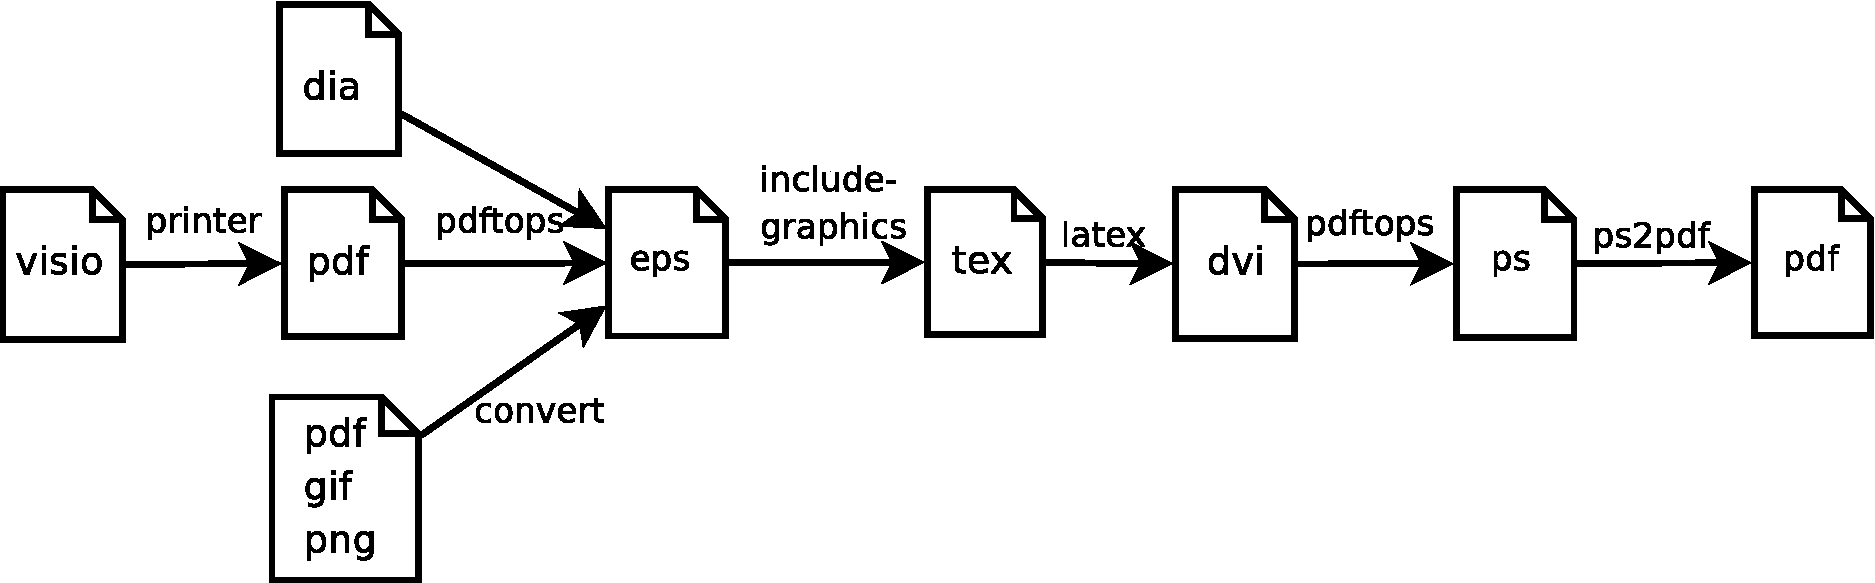
\includegraphics[scale=0.4]{pics/graphic_1}
		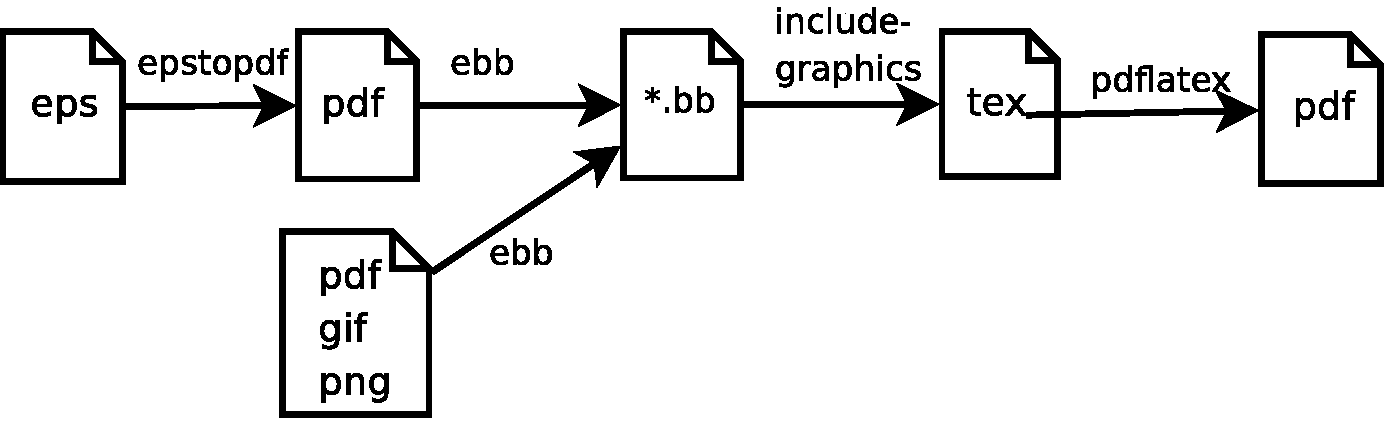
\includegraphics[scale=0.4]{pics/graphic_2} \\
		the text on the arrow is linux command and text in the frame is file format. The figure tell us that pdflatex, when used with graphics or graphicx packages, can compile correctly PNG and JPG files into DVI or PDF, but is not able to handle EPS files. Conversely, the precess of compiling with Latex to DVI and converting to PS and eventually PDF does support EPS, but doesn't supprot PNG and JPG.
		
		\item \linuxcommand{convert} is a command in ImageMagick tool package, the other commands are \linuxcommand{Identify} and \linuxcommand{combine}
		\item \linuxcommand{giftopnm myfile.gif >myfile.pnm} \linuxcommand{pnmtopng myfile.pnm myfile.png} png is new format file in internet. and pnm is intermediate format. Here I want to change gif file to png format.
		\item you can use \linuxcommand{less *.eps} to see if there is Boundbox defination.
		\item okular can view a lot of file format: pdf, ps ,dvi
		\end{itemize}
\section{math}
		\subsection{text in math}
			\begin{itemize}
			\item any space and newline has no meaning in math enoriment. you need specific command to produce space \\
				\begin{tabular}{|c|c|c|}
				\hline \verb=\,= & small space & = 3/18 of a quad \\
				\hline \verb=\:= & medium  & = 4/18 of a quad \\
				\hline \verb=\;= & large space  & = 5/18 of a quad\\
				\hline \verb=\!= & negative space  & = -3/18 of a quad\\
				\hline
				\end{tabular}
			\item What's difference between \verb=\textrm= and \verb=\mathrm= ? \\
			\verb=\[ a^\mathrm{a}_\textrm{a} \]=  will produce \[ a^\mathrm{a}_\textrm{a} \]
			can you see the diffence? the \verb=\mathrm= can change size with different postion. \verb=\textrm= is static.
			\end{itemize}
		
		\subsection{equation}
		\begin{enumerate}
		\item Simple variables are represented by italic letters, as $a b c x y z$.
		\item Vectors are written in bold face italic, as $\boldsymbol{B}$.
		\item Tensors of 2nd order and matrices may appear in a sans serif font, as
		M D I.
		\item The special numbers e, i, $\pi$, as well as the differential operator d, are to be
		written in an upright font to emphasize that they are not variables.
		\item A measurement consisting of a number plus a dimension is an indivisible
		unit, with a smaller than normal space between them, as 5.3 km and 62 kg.
		The dimension is in an upright font.
		\end{enumerate} \par

		here is two kind of formulas, text and displayed mode, the text mode exist within a line, so it don't need a equation number. (It's very easy to understand it), fractoin should be written to $a/b$ in text mode. \\	
		\[ \left\{
		\begin{array}{l}
		\textrm{text mode}	\left\{
					\begin{array}{l}
					\verb=\begin{math}...\end{math}= \\
					\verb=\(...\)= \\
					\verb=$...$=\\
					\end{array}
					\right. \vspace{2ex} \\
									
		\textrm{displayed mode}	\left\{
					\begin{array}{l}
					\textrm{number:  } \verb=\begin{equation}...\end{equation}= \\
					\textrm{no number}	\left\{
								\begin{array}{l}
								\verb=begin{displaymath}...\end{..}= \\
								\verb=\[...\]= \\
								\verb=$$...$$= \\
								\end{array}
								\right. \vspace{1ex} \\
					\end{array}
					\right.\\
		\end{array}
		\right. \]
		
		size of symbol in formula \\
		\begin{tabular}{|c|c|}
		\hline \verb=\displaystyle= & displayed formulas\\
		\hline \verb=\textstyle= & text formulas\\
		\hline \verb=\scriptstyle= & first sub-, superscript\\
		\hline \verb=\scriptscriptstyle= & later sub-, superscripts\\
		\hline
		\end{tabular} \\
		
		font will change according to the postion. \\
		\begin{tabular}{|c|c|c|c|}
		\hline active size & upper & lower & subscripts\\
		\hline D & T & T & S\\
		\hline T & S & S & S\\
		\hline S & SS & SS & SS\\
		\hline SS & SS & SS & SS\\
		\hline
		\end{tabular}

		\verb=\[ a_0 + \frac{1}{a_1 + \frac{1}{a_2 + \frac{1}{a_3 + \frac{1}{a_4}}}} \]=
		\[ a_0 + \frac{1}{a_1 + \frac{1}{a_2 + \frac{1}{a_3 + \frac{1}{a_4}}}} \]

		\begin{verbatim}
		\[ a_0 +
		\frac{1}{\displaystyle a_1 +
		\frac{1}{\displaystyle a_2 +
		\frac{1}{\displaystyle a_3 +
		\frac{1}{a_4}}}}
		\]
		\end{verbatim}
		will output
		\[ a_0 +
		\frac{1}{\displaystyle a_1 +
		\frac{1}{\displaystyle a_2 +
		\frac{1}{\displaystyle a_3 +
		\frac{1}{a_4}}}}
		\]
		array enviromnet is T \\
		D and T only difference in some symbol, such as \verb=\int \sum= \\
		\subsection{example}
			\begin{itemize}
			\item There is many kind of dots \verb=\ldots \cdots \vdots \ddots=, guess what they mean? Only \verb=\ldots= is allowed in normal text mode.
			\item text in formula should be put into \verb=\mbox{text}=
			\item \verb=\[ \oint\limits^\infty_0 \]= will produce \[ \oint\limits^\infty_0 \]
				\verb=\[ \oint^\infty_0 \]= produce \[ \oint^\infty_0 \]
				can you see the diffence with \verb=\limits=?
			\item \verb=\[ \underbrace{a + \overbrace{b + \cdots + y}^{123} + z}_{\alpha\beta\gamma} \]=
				\[ \underbrace{a + \overbrace{b + \cdots + y}^{123} + z}_{\alpha\beta\gamma} \]
				the same function include \verb=\underline \overline=
			\item  \verb!$ \vec{x} \stackrel{\mathrm{def}}{=} (x_1)$! will produce
				$ \vec{x} \stackrel{\mathrm{def}}{=} (x_1$
			\item  \verb=\begin{eqnarray}= means lines thus have the same behavior as they would in a \verb=\be gin{array} {rcl}. . . \end{array}= environment.
			\item
				\begin{verbatim}
				\begin{displaymath}
				{}^{12}_{\phantom}{1}6}\textrm{C} \qquad \textrm{versus}
				\qquad {}^{12}_6}\textrm{C}
				\end{displaymath}
				\end{verbatim}
				
				\begin{displaymath}
				{}^{12}_{\phantom{1}6}\textrm{C} \qquad \textrm{versus}
				\qquad {}^{12}_6\textrm{C}
				\end{displaymath}
			\item
				\begin{verbatim}
				\parbox{4cm}{\begin{eqnarray} \alpha &=& f(z)...\end{eqnarray}}
				\hfill \parbox{2.5cm}{\begin{eqnarray*}
				x &=& \alpha^2 - \beta^2\\ y &=& 2\alpha\beta \end{eqnarray*}}
				\hfill \begin{minipage}{4.5cm} The left-hand ... \end{minipage}
				\end{verbatim}
				
				\parbox{4cm}{\begin{eqnarray} \alpha &=& f(z)...\end{eqnarray}}
				\hfill \parbox{2.5cm}{\begin{eqnarray*}
				x &=& \alpha^2 - \beta^2\\ y &=& 2\alpha\beta \end{eqnarray*}}
				\hfill \begin{minipage}{4.5cm} The left-hand forumula is produce by parbox and minipage,you can learn from source code \end{minipage}
			\item
			\verb=\mathbf= produce bold, but upright, if you want to get italic, use \verb=\boldsymbol=
			\item
			\begin{verbatim}
				\begin{eqnarray}
				(x+y)(x-y) & = & x^2-xy+xy-y^2 \nonumber\\
				& = & x^2 - y^2 \\
				(x+y)^2
				& = & x^2 + 2xy + y^2
				\end{eqnarray}
			\end{verbatim}
			whill produce this
			\begin{eqnarray}
			(x+y)(x-y) & = & x^2-xy+xy-y^2 \nonumber\\
			& = & x^2 - y^2 \\
			(x+y)^2
			& = & x^2 + 2xy + y^2
			\end{eqnarray}

			\item \verb=\[\fbox{$\displaystyle \int^\infty_0 f(x)\,\mathrm{d}x ..$}\]=
				\[\fbox{$\displaystyle \int^\infty_0 f(x)\,\mathrm{d}x ..$}\]
			
			\item
			\verb=\substack{1st line\\2nd line\\...\\ last line}= \\
			\verb=\begin{subarray}{pos} 1st line\\2nd line\\...\\ last line \end{subarray}= \\
			\verb=\[ \sum_{\begin{subarray}{l} i\in\Lambda\\ i<j<n \end{subarray}} P(i,j) \]= produce
			\[ \sum_{\begin{subarray}{l}i\in\Lambda\\ i<j<n\end{subarray}} P(i,j) \]
			\end{itemize}
\section{table}
	\subsection{style parameters}
			\begin{description}	
			\item [\textbackslash{}tabcolsep] is half the width of the spacing that is inserted between columns in the tabular and tabular* environments;
			\item [\textbackslash{}arraycolsep] is the corresponding half intercolumn spacing for the array environment;
			\item [\textbackslash{}arrayrulewidth] is the thickness of the vertical and horizontal lines within a table;
			\item [\textbackslash{}doublerulesep] is the separation between the lines of a double rule.
			\end{description}
	
			Changes in these parameters can be made with the \verb=\setlength= command as usual. For example, to make the line thickness to be 0.5 mm, give \verb=\setlength{\arrayrulewidth}{0.5mm}= Furthermore, the parameter \verb=\arraystretch= can be used to change the distance between the rows of a table. This is a multiplying factor, with a standard value of 1. A value of 1.5 means that the inter-row spacing is increased by 50\%. A new value is set by rede?¨?ning the parameter with the command \linebreak[4] \verb=\renewcommand{\arraystretch}{factor}= \par
		\subsection{example}
			An example is listed below, It give common trip to create a table, It's enough for common useage. if you need more, you can find in the \cite{Companion}.
			\begin{verbatim}
			\begin{tabular}{|r|l||rrr|r@{:}l|r@{:}l||c|}\hline
			\multicolumn{10}{|c|}{\bfseries 1st Regional Soccer League
			Final Results 2002/03}\\ \hline
			&\itshape Club &\itshape W &\itshape T &\itshape L &
			\multicolumn{2}{c|}{\itshape Goals}
			& \multicolumn{2}{c||}{\itshape Points}
			& \itshape Remarks \\ \hline\hline
			
			1& Kingston Cowboys & 13 & 6 & 14
			& 54&45 & 32&34 & Medium Teams \\
			2 & Daysdon Bombers & 14 & 10
			& 9 & 66 & 50 & 38 & 28 & \\ \cline{1-9}
			3& Ralston Regulars & 3 & 11& 19 & 37&74 &
			17&49 & \raisebox{1.5ex}[0pt]{Demoted}\\ \hline
			\end{tabular}
			\end{verbatim}
			
			\begin{tabular}{|r|l||rrr|r@{:}l|r@{:}l||c|}\hline
			\multicolumn{10}{|c|}{ \rule[-3mm]{0mm}{8mm} \bfseries 1st Regional Soccer League
			Final Results 2002/03}\\ \hline
			&\itshape Club &\itshape W &\itshape T &\itshape L &
			\multicolumn{2}{c|}{\itshape Goals}
			& \multicolumn{2}{c||}{\itshape Points}
			& \itshape Remarks \\ \hline\hline
			
			1& Kingston Cowboys & 13 & 6 & 14 & 54&45 & 32&34 & Medium Teams \\ \hline
			2 & Daysdon Bombers & 14 & 10 & 9 & 66 & 50 & 38 & 28 & \\ \cline{1-9}
			3& Ralston Regulars & 3 & 11 & 19 & 37&74 & 17&49 & \raisebox{1.5ex}[0pt]{Demoted}\\ \hline
			\end{tabular}
			There are some notes you should know from the previous example.
			\begin{itemize}
			\item you need to understand \verb=@{:}=
			\item \verb=\rule[-3mm]{0mm}{8mm}= make the
head row higher to make it look
nice。Just like a expander, width is 0, so it's invisible, -3mm represent the expand the below.

			\item \verb=\raisebox= to lift the text in the last row
			\item \verb=\mulitcolumn= and \verb=cline= to make complex appearance.
			\end{itemize}

\section{User define}
	\subsection{add other .sty}
	if you can find a file.sty, copy it to tex distribution path, if It's package, maybe you need run latex command such as latex acrotex.ins. don't forget use texhash command in the end to update the search database.
	
	\subsection{counter and length}
			\[ \left\{ \begin{array}{lll}
				\textrm{counter}: \frame{\parbox{10em}{part, chapter,  section, paragraph,  page, equation, table enumi}} & \left\{ \begin{array}{ll} \textrm{change} & \left\{ \begin{array}{l}
													\verb=\setcounter= \\
													\verb=\addtocounter= \\	
													\verb=\stepcounter= \\
													\verb=\refstepcounter= \\	
												\end{array}
												\right.\\
										\textrm{user def} & \verb=\newcounter=  \\
										\textrm{custom} & \left\{ \begin{array}{l}
													 \verb=\new=\emph{counter}  \\
													\verb=\arabic= \\
													\verb=\alph= \\	
												\end{array}
												\right.
							\end{array}
						\right. \\
				\textrm{length}: \parbox{10em}{\textbackslash{}parskip, \textbackslash{}textwidth } & \left\{ \begin{array}{ll} \textrm{change} & \left\{ \begin{array}{l}
													\verb=\setlength= \\
													\verb=\addtolength= \\	
													\verb=\settowidth= \\
													\verb=\settoheight= \\
													\verb=\settodepth= \\	
												\end{array}
												\right.\\
										\textrm{user def} & \verb=\newlength=  \\
							\end{array}
						\right. \\
				\end{array}
			\right. \] \\
			\verb=\newcounter{zypage}= \\
			\verb=\setcounter{zypage}{\value{page}}= \\
			a good example is \verb=\renewcommand{\thesection}{\Alph{section}}= \\
			\begin{verbatim}
			\newlength{\zywdth}
			\newcommand{\zydefbox}[1]{\settowidth{\zywdth}{#1}}
			\newcommand{\zytextbox}[1]{\framebox[\zywdth]{#1}}
			\end{verbatim}
	\subsection{command}
		\begin{description}
		\item[Definition]:
			\begin{verbatim}
			\newcommand{\com_name}[narg][opt]{def}
			\renewcommand{\om_name}[narg][opt]{def}
			\end{verbatim}
		\item[Example]:
			\begin{verbatim}
			 \newcommand{\subvec}[3][x]{\ensuremath{#1_{#2},\ldots,#1_{#3}}}
			\end{verbatim}
			 \newcommand{\subvec}[3][x]{\ensuremath{#1_{#2},\ldots,#1_{#3}}}
			now \verb=\subvec{i}{j}= will produce
			\subvec{i}{j}. here. \verb=\ensuremath= to make
it applicable both in text and in
math.if \verb=\subvec[a]{i}{j}= produce \subvec[a]{i}{j}.
If you provide, use default, If you provide, use what you provide.  pay attention to [a], If you don't have optional argument, you have to use \verb=\subver{x}{i}{j}= command.

%也就是说,如果你不提供,那么就使用默认的,如果你提供,
%那么就是用你提供的。这里注意,用方括号[a]。如果没有这个optional参数,你就必须用\verb=\subver{x}{i}{j}=命令。
		\end{description}
		
	 \subsection{enviroment}.
		\begin{description}
		\item[Definition]:
			\begin{verbatim}
			\newenvironment{\env_name}[narg][opt]{beg_def}{end_def}
			\renewenvironment{\env_name}[narg][opt]{beg_def}{end_def}
			\end{verbatim}
		\item[Example]:
			\begin{verbatim}
			\newcounter{com}
			\newsavebox{\comname}
			\newenvironment{ZYcommnet}[1][zhao yan]
			{\begin{sloppypar}\noindent\stepcounter{com}\slshape
			Comment \arabic{com} \sbox{\comname}{#1}
			\begin{quote}\small\itshape}

			 {\hspace*{\fill}\usebox{\comname}\end{quote}\end{sloppypar}}
			\end{verbatim}
		
			\newcounter{com}
			\newsavebox{\comname}
			\newenvironment{ZYcomment}[1][zhao yan]
			{\begin{sloppypar}\noindent\stepcounter{com}\slshape
			Comment \arabic{com} \sbox{\comname}{#1}
			\begin{quote}\small\itshape}
			 {\hspace*{\fill}\usebox{\comname}\end{quote}\end{sloppypar}}

        \begin{verbatim}
          \begin{ZYcomment}[ZhaoYan]
			Any thing can be finished by you hard work...
			\end{ZYcomment}
        \end{verbatim}
		will produce: \\	
			\begin{ZYcomment}[ZhaoYan]
			Any thing can be finished by you hard work...
			\end{ZYcomment}
		\end{description}

\section{Ebook and html}
\begin{itemize}

\item There are three kinds of outputs:
\begin{enumerate}
	\item pdf version for printed book.  
	\item tex4ebook to produce epub book.
	\item tex4ebook also produces html result.
\end{enumerate}

\item For pdf version:

\item For epub:
\begin{enumerate}
	\item Change Hilight command to empty. Because it doesn't support hight light command.
\begin{verbatim}
%\newcommand{\Hilight}[1]{\makebox[0pt][l]{\color{yellow}\rule[-3pt]{#1em}{11pt}}}
%\newcommand{\HilightLine}[2][yellow]{\makebox[0pt][l]{\color{#1}\rule[-4pt]{#2em}{13.9pt}}}

\newcommand{\Hilight}[1]{}
\newcommand{\HilightLine}[2][yellow]{}
\end{verbatim}
\item use tex4ebook, it will output all files to current directory, \textbf{it based on make4ht}
\verb|tex4ebook -c config_kindle.cfg -d ebook |

\item For html: You can also use tex4eboo, but use the different config_html.cfg
\begin{enumerate}
	\item it uses "pics/visitor.png", if you want to copy all the content to your website, don't forget copy all the pics directory.
\end{enumerate}

\end{enumerate}

\item Use MacTex, \textbf{You should download full set, Don use basic installation package about 2G}, Because when you install make4ht, you need install a lot of extra package, it's not very convenient. If you space is too limited, you can use tex live utility tool to help you download and install package. 

\item In mac, you need to edit .bash\_profile and edit \$PATH
\begin{verbatim}
export PATH=$PATH:/Library/TeX/texbin
\end{verbatim}

\item download make4ht, unzip and come into unzipped directory. 
\verb=make, and make install"=

\item Go to cpp directory, build config.cfg file and write these contents to it. \textbf{No empty line in this config.cfg, or make4ht will report error.}
\begin{verbatim}
\Preamble{xhtml}
\Css{
body{font-size:1.3em;}
li {
    margin: 0;
    padding: 0.2em;
}
div.lstlisting{
    background-color: rgb(233,233,233); 
    border-style: double;
}
}
\begin{document}
\EndPreamble

\end{verbatim}

\begin{verbatim}
make4ht -d html -c config.cfg cpp.tex "html,index=3,5,next, section+, charset=utf-8" 
\end{verbatim}

\item It will produce all the html file in the directory. Copy this html directory to zhaoyan.website.  Then You can copy all the html file and pics directory to zhaoyan.website. 

\item You need to add header.html and side.html to cpp.html

\item  add below before </head>
\begin{verbatim}
<link href="/css/whole.css" rel="stylesheet" type="text/css" />    
    
</head><body 
>
\end{verbatim}

\item add below 

\begin{verbatim}
<div id="maincontent"  >

<div align="center"  style="float: left; width:55%; ">
<a href="cpp.html">C++ language</a> &nbsp; &nbsp; <a href="../algorithem.php">Algorithm</a>  &nbsp; &nbsp; <a href="../design.php">Design pattern</a> &nbsp; &nbsp;
</div> <br />

<p>In this part I will mainly introduce some valuable C++ knowledge. All these knowledge is summaried by <a href="/index.php">me</a> from my reading and develping caree. And this part will be updated continously.</p>


<p>All the links below have been published in the book <a href="http://www.amazon.com/Drops-knowledge-Practical-Skills-using-ebook/dp/B01ETXWMKO?ie=UTF8&*Version*=1&*entries*=0"> "Drops of knowledge of C++"</a>. It can be purchased with $0.99 and downloaded to you Kindle reader </p> 

\end{verbatim}

\item change 

\begin{verbatim}
change
 <div class="tableofcontents" >
to
 <div class="tableofcontents" align="left">
\end{verbatim}





\item download tex4ebook for kindle format book
\verb=make, and make install"=
go to your tex directory, and change your pics/fig to pics/fig.png. You need to give extension name here.
\verb=tex4ebook cpp.tex=. It will produce a cpp-epub directory. Then you can upload cpp.epub to amazon website.


		
\end{itemize}
\section{Error}
\begin{itemize}
 \item I made a typo erro with double right parentheses \verb=\begin{tabular}{|c|c|}}=
  When I click pdflatex in kile menu, There is no output in log windows, then I run pdflatex in terminal,
  found that compiling has been suspended. I have to ctrl+Z to stop it. there are two conclusions: terminal command is better and compiling sometimes will be suspended, be careful for that.
 \item Some errors can be resolved by run PDFLatex command more than once, try 2 or 3 times.
 \item When I use listings package, use pdflatex compile it, no error, but no pdf is produced. When you switch to command prompt, use command pdflatex cpp.tex, it prompt to install listings package. I think that you can try use administer to run the WinEdt . Or you can use command interface when you meet this questions again. In windows, \textbf{It's important to use administer to run VS , WinEdt  or other applications}
\item miktex can install package on the fly, but you need run WinEdt by administer. texlive can't install package automatically, You can use \linuxcommand{tlmgr install url} to install url.sty. You don't need give .sty in the command.If tlmgr doesn't work,  maybe you need \linuxcommand{sudo apt-get install xzdec}. I don't know what it means
    \item  in Mint, you can sue software manager to install texlive-font-recommend and latex-recommend two extra package to resolve most missing package and font problem.
    \item In linux, If you use texmaker or kile, when you compile fail,  the process is still run. it make some files, such as  book.aux is written protected.Before you compile again, you need to delete them manually.
    \item if you \verb=\textbf{...= forget right \} symbol, in line 100. maybe error message show there is werid error in line 1000. this information is not very useful. So you need to take a look a .log file. and see what line is analyzed  before line 1000. Maybe it show it's dealing with line 100, It's very helpful information. 
\end{itemize}



\ifx \allfiles \undefined
\bibliography{../book}
%\end{CJK*}
\end{document}
\fi
